% Created by tikzDevice version 0.10.1 on 2016-02-27 13:20:05
% !TEX encoding = UTF-8 Unicode
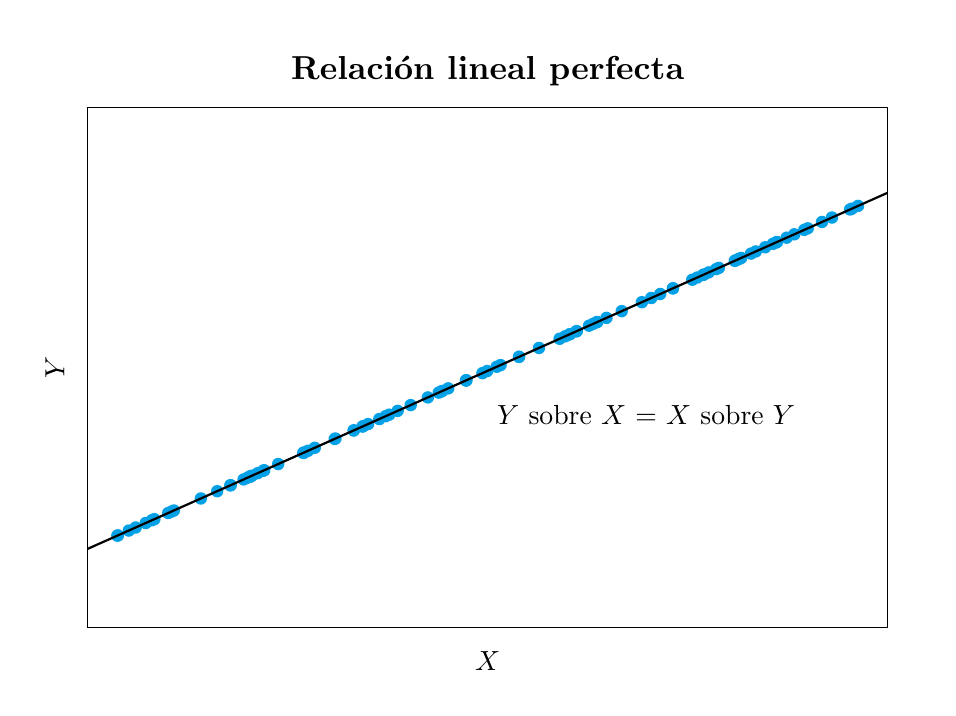
\begin{tikzpicture}[x=1pt,y=1pt]
\definecolor{fillColor}{RGB}{255,255,255}
\path[use as bounding box,fill=fillColor,fill opacity=0.00] (0,0) rectangle (325.21,238.49);
\begin{scope}
\path[clip] ( 21.68, 21.68) rectangle (310.76,209.58);
\definecolor{fillColor}{RGB}{5,161,230}

\path[fill=fillColor] (170.88,116.57) circle (  2.25);

\path[fill=fillColor] (177.53,119.53) circle (  2.25);

\path[fill=fillColor] ( 50.79, 63.12) circle (  2.25);

\path[fill=fillColor] ( 32.62, 55.02) circle (  2.25);

\path[fill=fillColor] (111.23, 90.02) circle (  2.25);

\path[fill=fillColor] (246.09,150.05) circle (  2.25);

\path[fill=fillColor] (266.49,159.13) circle (  2.25);

\path[fill=fillColor] (255.80,154.38) circle (  2.25);

\path[fill=fillColor] (148.53,106.62) circle (  2.25);

\path[fill=fillColor] ( 62.58, 68.36) circle (  2.25);

\path[fill=fillColor] ( 32.39, 54.92) circle (  2.25);

\path[fill=fillColor] ( 80.30, 76.25) circle (  2.25);

\path[fill=fillColor] (198.23,128.75) circle (  2.25);

\path[fill=fillColor] (228.57,142.26) circle (  2.25);

\path[fill=fillColor] (297.17,172.79) circle (  2.25);

\path[fill=fillColor] (101.29, 85.59) circle (  2.25);

\path[fill=fillColor] (184.76,122.75) circle (  2.25);

\path[fill=fillColor] (127.05, 97.06) circle (  2.25);

\path[fill=fillColor] (209.14,133.61) circle (  2.25);

\path[fill=fillColor] ( 99.88, 84.97) circle (  2.25);

\path[fill=fillColor] (277.02,163.82) circle (  2.25);

\path[fill=fillColor] ( 83.08, 77.49) circle (  2.25);

\path[fill=fillColor] (133.69,100.02) circle (  2.25);

\path[fill=fillColor] (123.00, 95.26) circle (  2.25);

\path[fill=fillColor] ( 52.00, 63.65) circle (  2.25);

\path[fill=fillColor] (202.86,130.81) circle (  2.25);

\path[fill=fillColor] (221.94,139.30) circle (  2.25);

\path[fill=fillColor] (255.50,154.24) circle (  2.25);

\path[fill=fillColor] (300.05,174.08) circle (  2.25);

\path[fill=fillColor] (164.33,113.66) circle (  2.25);

\path[fill=fillColor] (204.32,131.46) circle (  2.25);

\path[fill=fillColor] ( 45.77, 60.88) circle (  2.25);

\path[fill=fillColor] ( 80.54, 76.36) circle (  2.25);

\path[fill=fillColor] (257.83,155.28) circle (  2.25);

\path[fill=fillColor] ( 78.03, 75.24) circle (  2.25);

\path[fill=fillColor] (248.79,151.25) circle (  2.25);

\path[fill=fillColor] (270.78,161.04) circle (  2.25);

\path[fill=fillColor] (129.34, 98.08) circle (  2.25);

\path[fill=fillColor] (280.63,165.43) circle (  2.25);

\path[fill=fillColor] (195.95,127.73) circle (  2.25);

\path[fill=fillColor] (192.21,126.07) circle (  2.25);

\path[fill=fillColor] ( 52.84, 64.02) circle (  2.25);

\path[fill=fillColor] (151.97,108.15) circle (  2.25);

\path[fill=fillColor] (158.55,111.08) circle (  2.25);

\path[fill=fillColor] (256.72,154.79) circle (  2.25);

\path[fill=fillColor] (297.87,173.10) circle (  2.25);

\path[fill=fillColor] (263.10,157.63) circle (  2.25);

\path[fill=fillColor] ( 99.60, 84.84) circle (  2.25);

\path[fill=fillColor] ( 42.65, 59.49) circle (  2.25);

\path[fill=fillColor] (257.02,154.92) circle (  2.25);

\path[fill=fillColor] ( 79.42, 75.86) circle (  2.25);

\path[fill=fillColor] (225.33,140.81) circle (  2.25);

\path[fill=fillColor] ( 36.54, 56.77) circle (  2.25);

\path[fill=fillColor] ( 85.08, 78.38) circle (  2.25);

\path[fill=fillColor] (244.03,149.14) circle (  2.25);

\path[fill=fillColor] (158.39,111.01) circle (  2.25);

\path[fill=fillColor] ( 39.03, 57.88) circle (  2.25);

\path[fill=fillColor] (130.61, 98.64) circle (  2.25);

\path[fill=fillColor] (117.88, 92.98) circle (  2.25);

\path[fill=fillColor] (149.86,107.22) circle (  2.25);

\path[fill=fillColor] (261.37,156.85) circle (  2.25);

\path[fill=fillColor] (144.60,104.88) circle (  2.25);

\path[fill=fillColor] (205.84,132.14) circle (  2.25);

\path[fill=fillColor] (117.77, 92.93) circle (  2.25);

\path[fill=fillColor] (194.22,126.96) circle (  2.25);

\path[fill=fillColor] ( 68.49, 70.99) circle (  2.25);

\path[fill=fillColor] (198.43,128.84) circle (  2.25);

\path[fill=fillColor] (121.26, 94.49) circle (  2.25);

\path[fill=fillColor] (270.34,160.85) circle (  2.25);

\path[fill=fillColor] (233.15,144.29) circle (  2.25);

\path[fill=fillColor] ( 73.22, 73.10) circle (  2.25);

\path[fill=fillColor] (249.77,151.69) circle (  2.25);

\path[fill=fillColor] (103.73, 86.68) circle (  2.25);

\path[fill=fillColor] (120.96, 94.35) circle (  2.25);

\path[fill=fillColor] ( 80.43, 76.31) circle (  2.25);

\path[fill=fillColor] ( 85.48, 78.56) circle (  2.25);

\path[fill=fillColor] (214.66,136.06) circle (  2.25);

\path[fill=fillColor] ( 99.68, 84.88) circle (  2.25);

\path[fill=fillColor] (241.94,148.21) circle (  2.25);

\path[fill=fillColor] (281.87,165.98) circle (  2.25);

\path[fill=fillColor] ( 44.88, 60.48) circle (  2.25);

\path[fill=fillColor] (195.76,127.65) circle (  2.25);

\path[fill=fillColor] ( 81.05, 76.59) circle (  2.25);

\path[fill=fillColor] ( 90.53, 80.81) circle (  2.25);

\path[fill=fillColor] (290.62,169.88) circle (  2.25);

\path[fill=fillColor] (158.42,111.03) circle (  2.25);

\path[fill=fillColor] (177.57,119.55) circle (  2.25);

\path[fill=fillColor] (205.60,132.03) circle (  2.25);

\path[fill=fillColor] (110.95, 89.89) circle (  2.25);

\path[fill=fillColor] (138.40,102.11) circle (  2.25);

\path[fill=fillColor] ( 73.37, 73.17) circle (  2.25);

\path[fill=fillColor] (233.18,144.31) circle (  2.25);

\path[fill=fillColor] (240.15,147.41) circle (  2.25);

\path[fill=fillColor] (244.40,149.30) circle (  2.25);

\path[fill=fillColor] (149.31,106.97) circle (  2.25);

\path[fill=fillColor] (166.05,114.42) circle (  2.25);

\path[fill=fillColor] (274.27,162.60) circle (  2.25);

\path[fill=fillColor] (287.03,168.28) circle (  2.25);

\path[fill=fillColor] (169.50,115.96) circle (  2.25);

\path[fill=fillColor] (269.30,160.39) circle (  2.25);
\end{scope}
\begin{scope}
\path[clip] (  0.00,  0.00) rectangle (325.21,238.49);
\definecolor{drawColor}{RGB}{0,0,0}

\node[text=drawColor,anchor=base,inner sep=0pt, outer sep=0pt, scale=  1.20] at (166.22,219.84) {\bfseries Relación lineal perfecta};

\node[text=drawColor,anchor=base,inner sep=0pt, outer sep=0pt, scale=  1.00] at (166.22,  6.08) {$X$};

\node[text=drawColor,rotate= 90.00,anchor=base,inner sep=0pt, outer sep=0pt, scale=  1.00] at ( 13.28,115.63) {$Y$};
\end{scope}
\begin{scope}
\path[clip] (  0.00,  0.00) rectangle (325.21,238.49);
\definecolor{drawColor}{RGB}{0,0,0}

\path[draw=drawColor,line width= 0.4pt,line join=round,line cap=round] ( 21.68, 21.68) --
	(310.76, 21.68) --
	(310.76,209.58) --
	( 21.68,209.58) --
	( 21.68, 21.68);
\end{scope}
\begin{scope}
\path[clip] ( 21.68, 21.68) rectangle (310.76,209.58);
\definecolor{drawColor}{RGB}{0,0,0}

\path[draw=drawColor,line width= 0.8pt,line join=round,line cap=round] ( 21.68, 50.16) -- (310.76,178.84);

\node[text=drawColor,anchor=base,inner sep=0pt, outer sep=0pt, scale=  1.00] at (223.48, 94.97) {$Y$ sobre $X$ = $X$ sobre $Y$};
\end{scope}
\end{tikzpicture}
